\documentclass{beamer}
\usepackage[magyar]{babel}
\usepackage[utf8]{inputenc}
\usepackage{mathtools}
\usepackage{amsfonts}
\usepackage{color}
\mode<presentation>{ \usetheme{boxes} } 
\title{Szóreprezentációk folytonos vektortérben}
\AtBeginSection[]{
    \begin{frame}
    \frametitle{Outline}
    \tableofcontents[currentsection]
    \end{frame}
}

\begin{document}

\begin{frame}
  \titlepage
\end{frame}

\section{Bengio et al 2013: A Neural Probabilistic Language Model}
\begin{frame}
\frametitle{A dimenziók átka}
\begin{itemize}
\item A hagyományos nyelvmodellek (pl. n-gram alapúak)

\item általában 1-2 szónyi környezet

\item nem veszik figyelembe a hasonlóságot

\medskip

“The cat is walking in the bedroom” 

“A dog was running in a room”
\end{itemize}

\end{frame}

\begin{frame}
\frametitle{Elosztott reprezentáció}
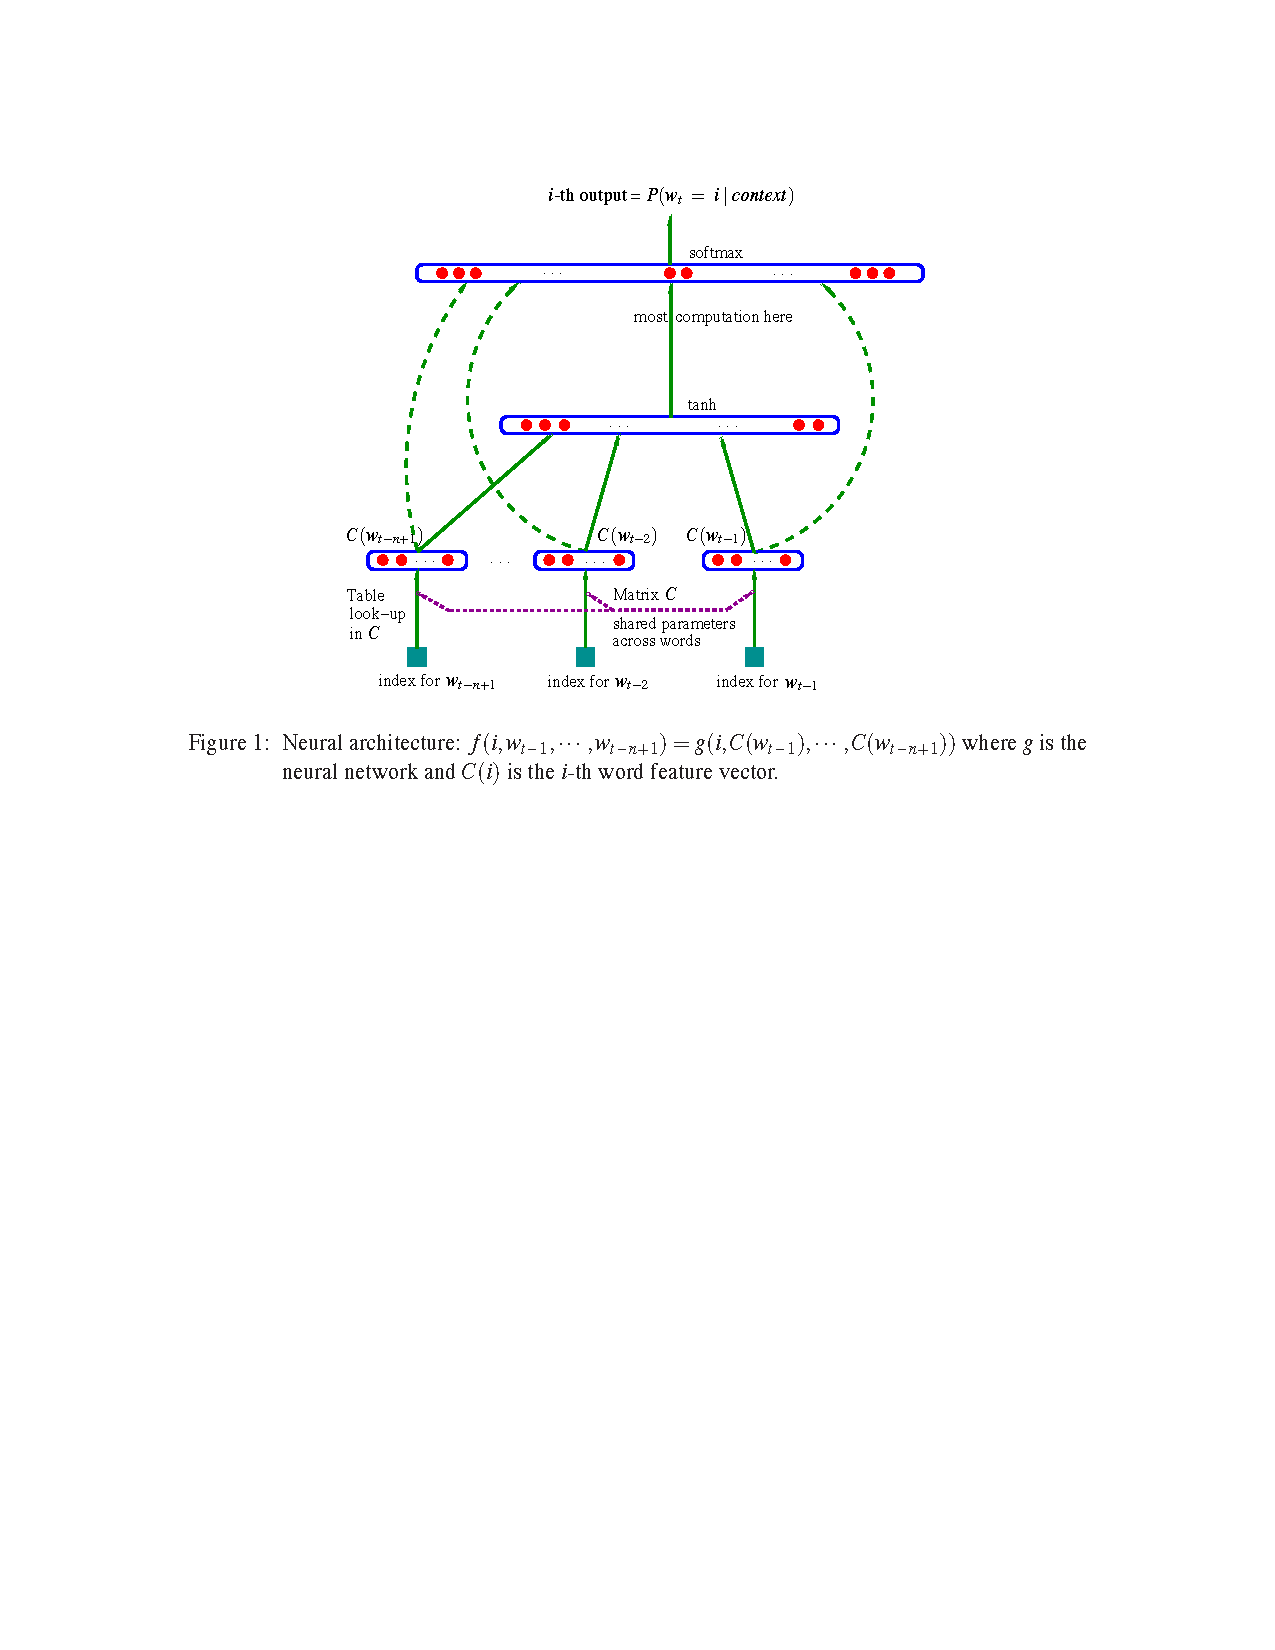
\includegraphics[width=\linewidth]{bengio-neural-archtecture.pdf}
\end{frame}

\begin{frame}

\begin{itemize}
\item Maximalizálni \[ L = \frac{1}{T} \sum_t \log f(w_t,w_{t-1},\dots,w_{t-n+1};\theta)+R(\theta) \]

\item Input \[ x = (C(w_{t-1}),C(w_{t-2}),\dots ,C(w_{t-n+1})) \]

\begin{itemize}
\item \( \dim(C) = \(|V| \times m\)
\end{itemize}

\item Output \[ y = b + W x + U \tanh(d + H x) \]

\begin{itemize}
\item \(\dim(b) = |V|\), \dim(W) = |V| \times (n-1)m, \dim(U) = |V| \times h, \dim(d) = h,
\dim(H) = h \times (n-1)m\) 
\end{itemize}

\item Normalizálás (softmax) \[ f(w_t,w_{t-1},\dots,w_{t-n+1}) = \frac{e^y_{w_t}}{\sum_i e^y_i} \]

\item Paraméterek száma \[ |V|(1+ nm + h) + h(1+(n-1)m) \]
\end{itemize}
\end{frame}

\begin{frame}
\frametitle{Eredmények}

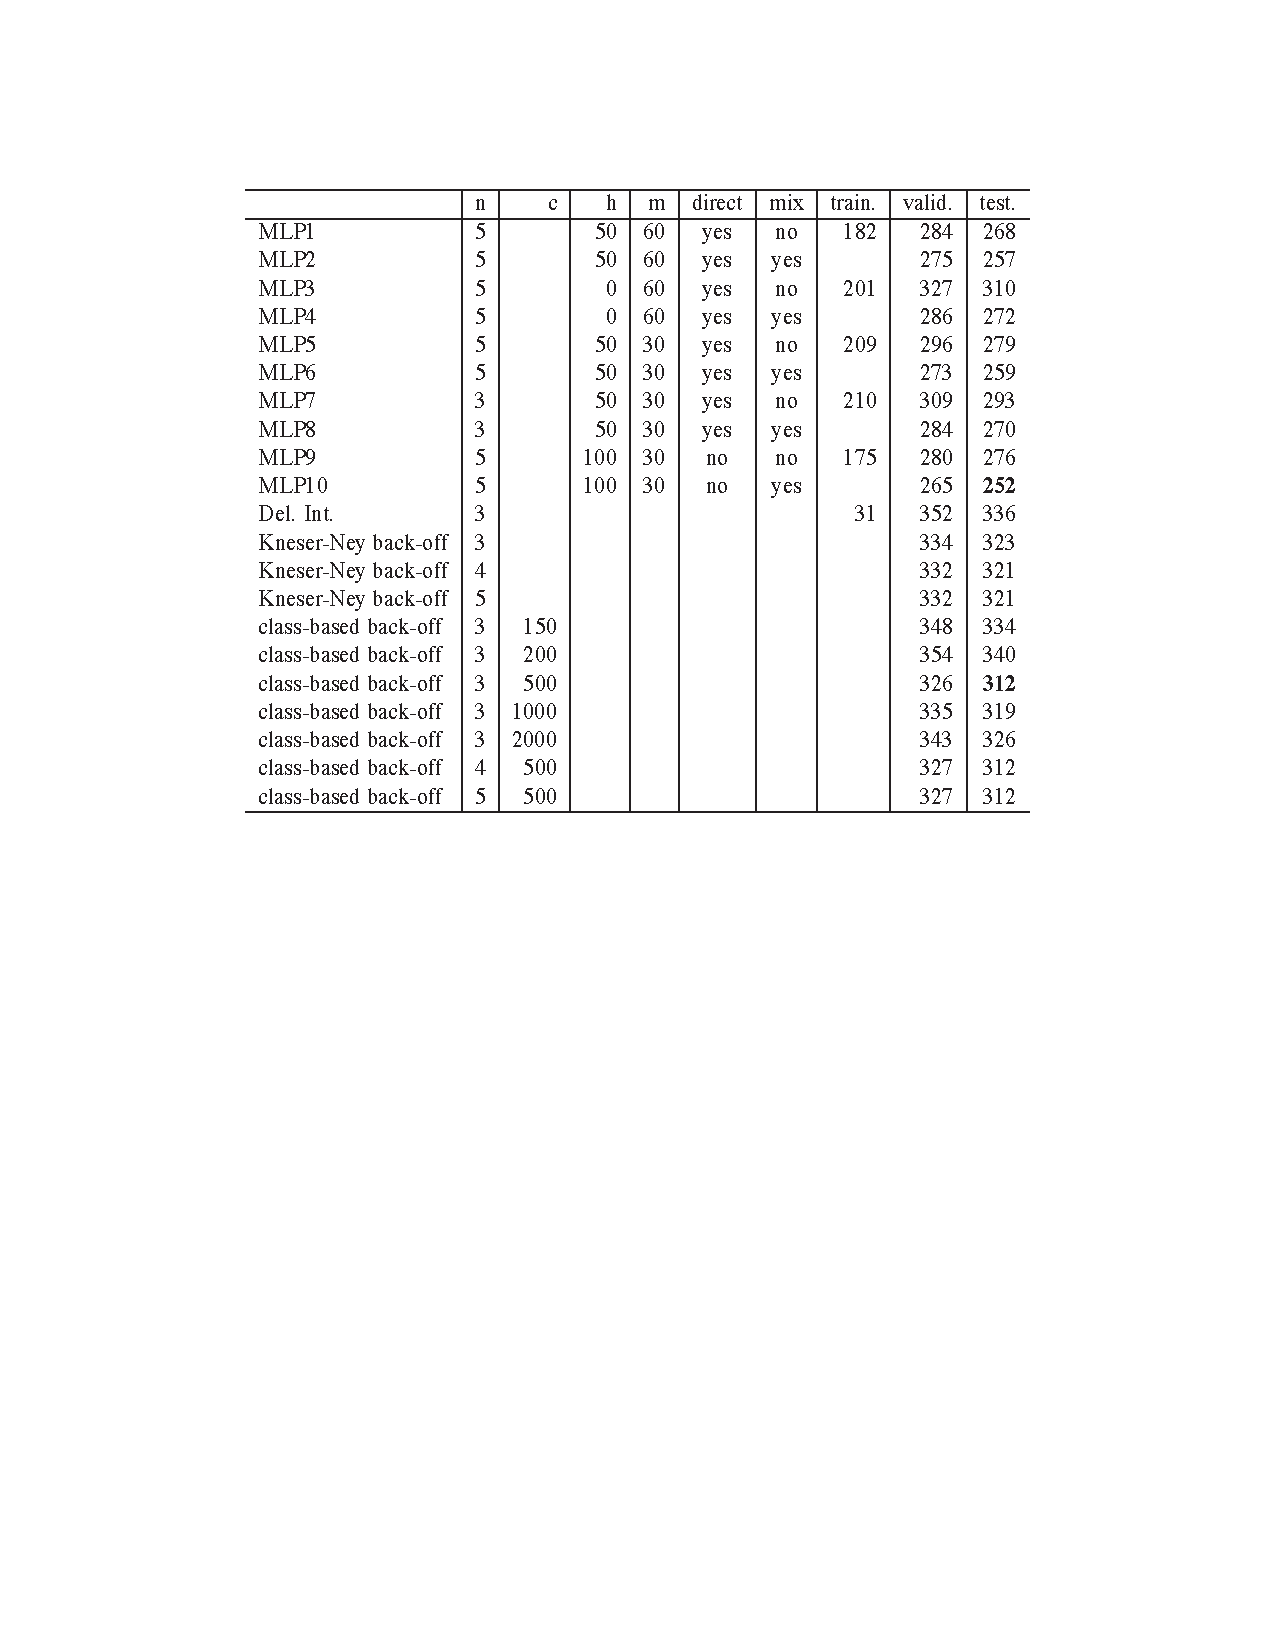
\includegraphics[width=\linewidth]{bengio-results.pdf}
\end{frame}

\section{Mikolov et al 2014: Efficient Estimation of Word Representation in Vector Space}
\begin{frame}
\begin{itemize}
\item Cél: jó minőségű szóvektorok tanulása

\item multiple degrees of similarity - szintakitikai és szemantikai

\[ v("King") - v("Man") + v("Woman") \sim v("Queen") \]
\end{itemize}

\end{frame}

\begin{frame}
\frametitle{Időköltségek}

\begin{itemize}
\item Feedforward Neural Net Language Model (NNLM)

\[ Q = n \times m + n \times m \times h + h \times |V| \]

bináris fa hierarchiába rendezve a szótárat \(\log_2(|V|)\)

\item Recurrent NNLM

\[ Q = h \times h + h \times |V| \]

Nincs projekciós réteg, \(m=h\)
\end{itemize}

\end{frame}

\begin{frame}
\frametitle{Egyszerűbb modellek szóvektortanulásra}

\begin{itemize}
\item Continuous Bag-of-Words

Szóvektorok átlagát veszi a környezetből, nincs rejtett réteg.

\[ Q = n \times m + m \times \log_2(|V|) \]

\item Continuous Skip-gram

1 szó az input, megjósolja a környező szavakat.

\[ Q = C \times (m + m \times \log_2(|V|) \]

\end{itemize}

\end{frame}

\begin{frame}
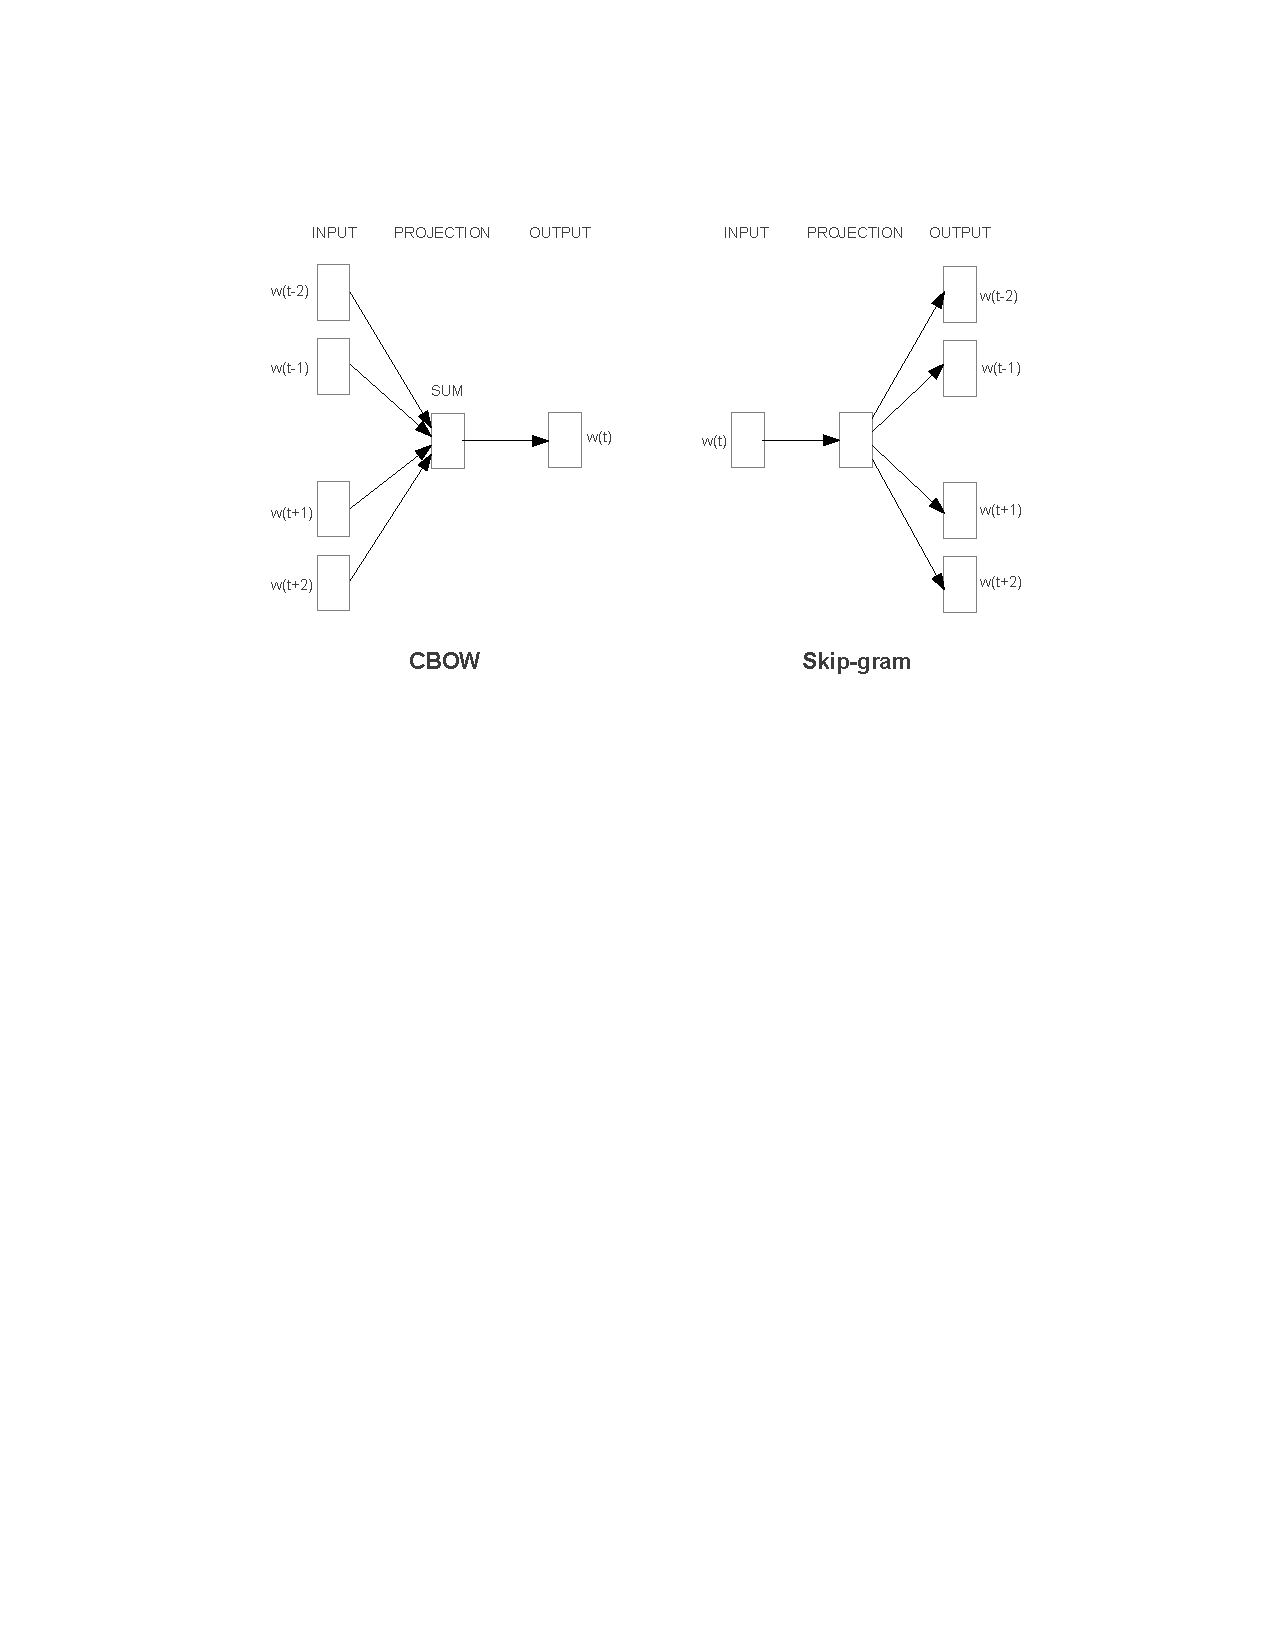
\includegraphics[width=\linewidth]{mikolov-cbow-skip}
\end{frame}


\begin{frame}
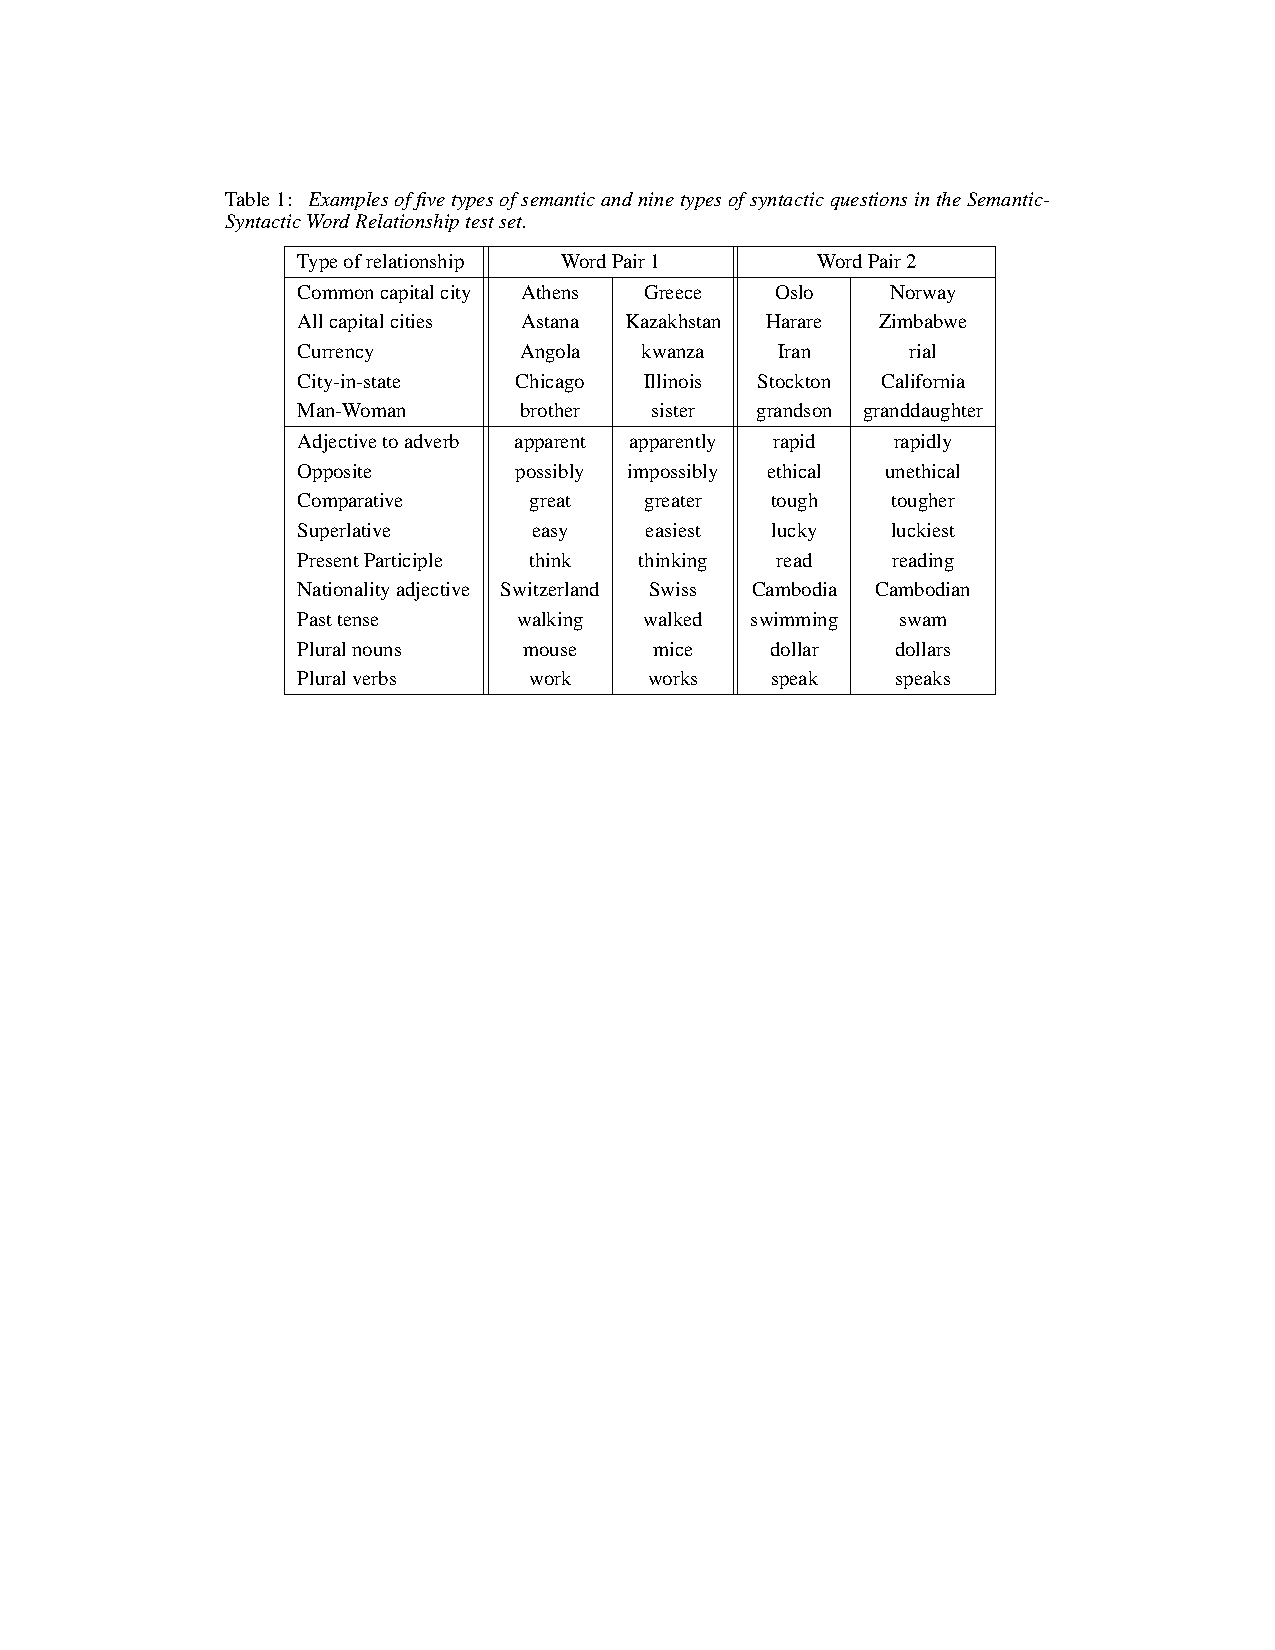
\includegraphics[width=\linewidth]{mikolov-test-set}
\end{frame}

\begin{frame}
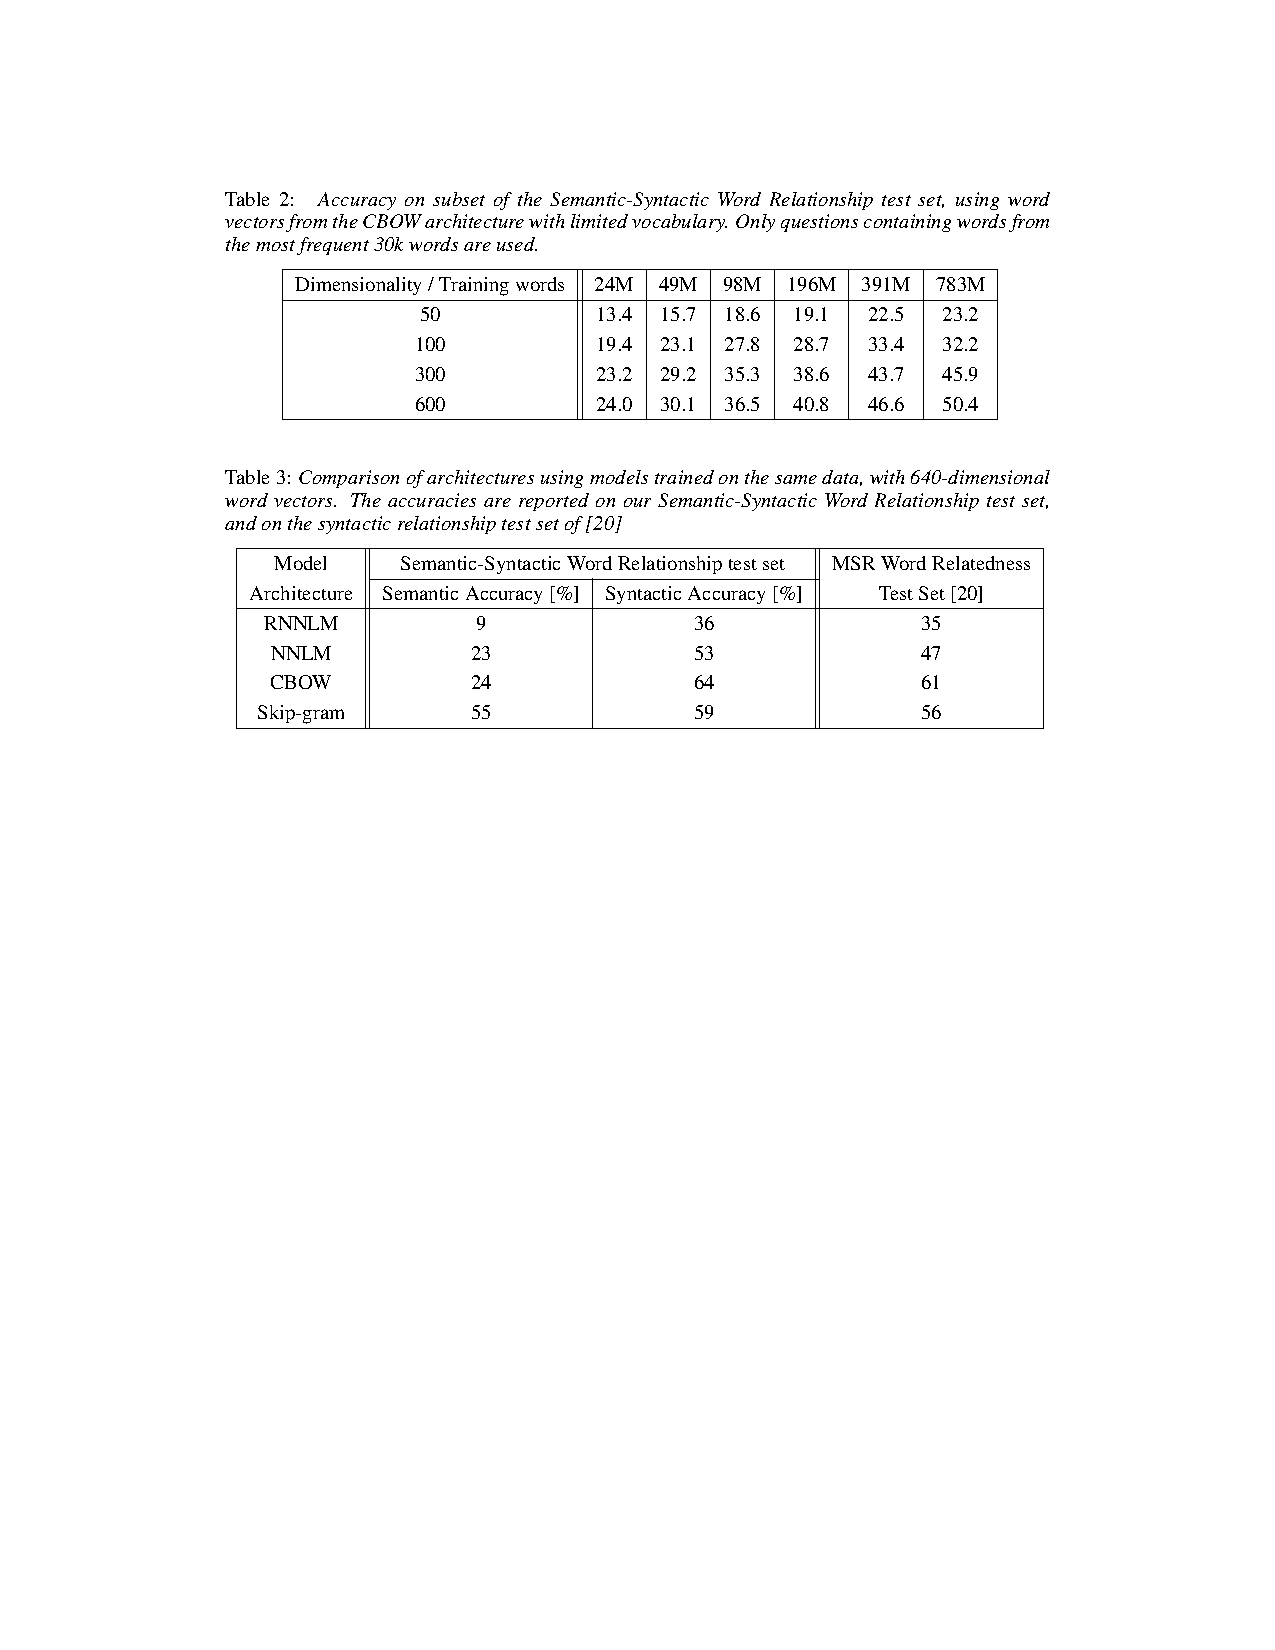
\includegraphics[width=\linewidth]{mikolov-results1}
\end{frame}

\begin{frame}
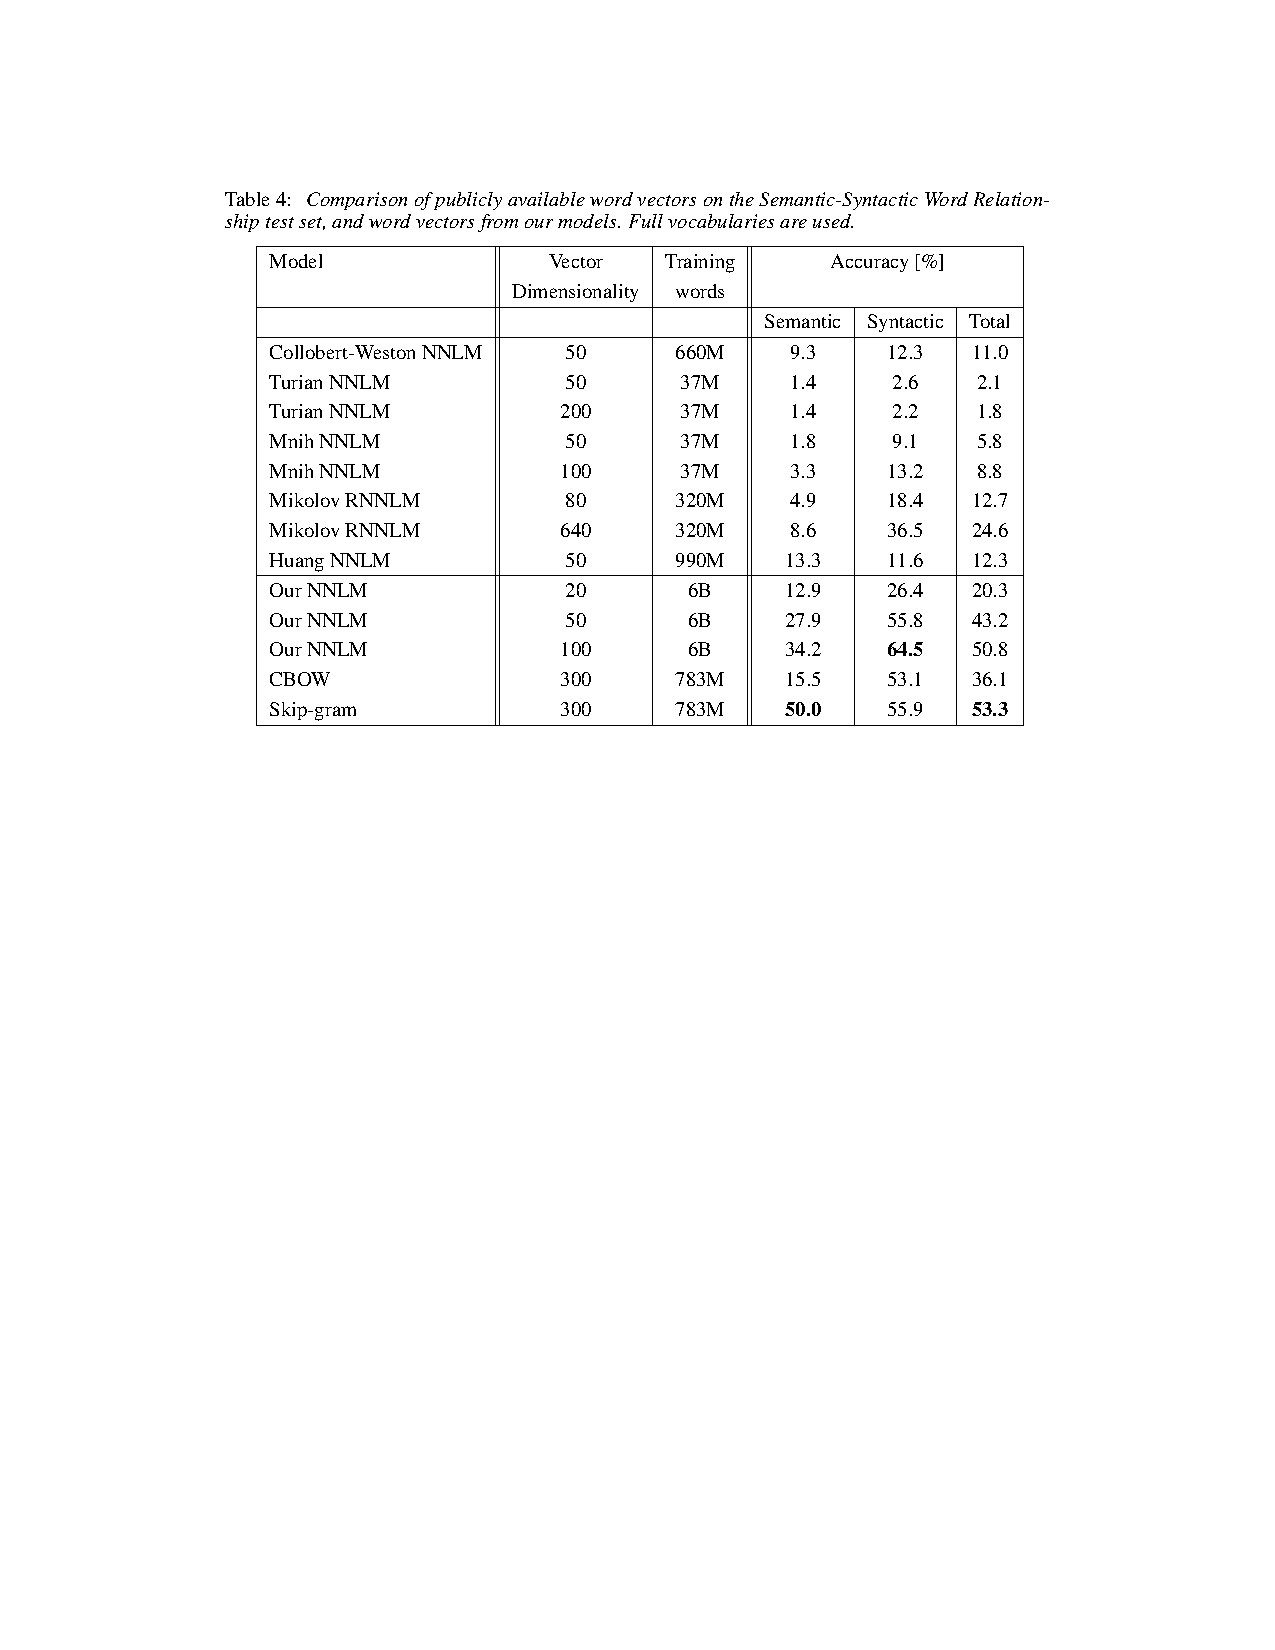
\includegraphics[width=\linewidth]{mikolov-results2}
\end{frame}

\begin{frame}
\includegraphics[width=\linewidth]{mikolov-training-time}
\end{frame}

\begin{frame}
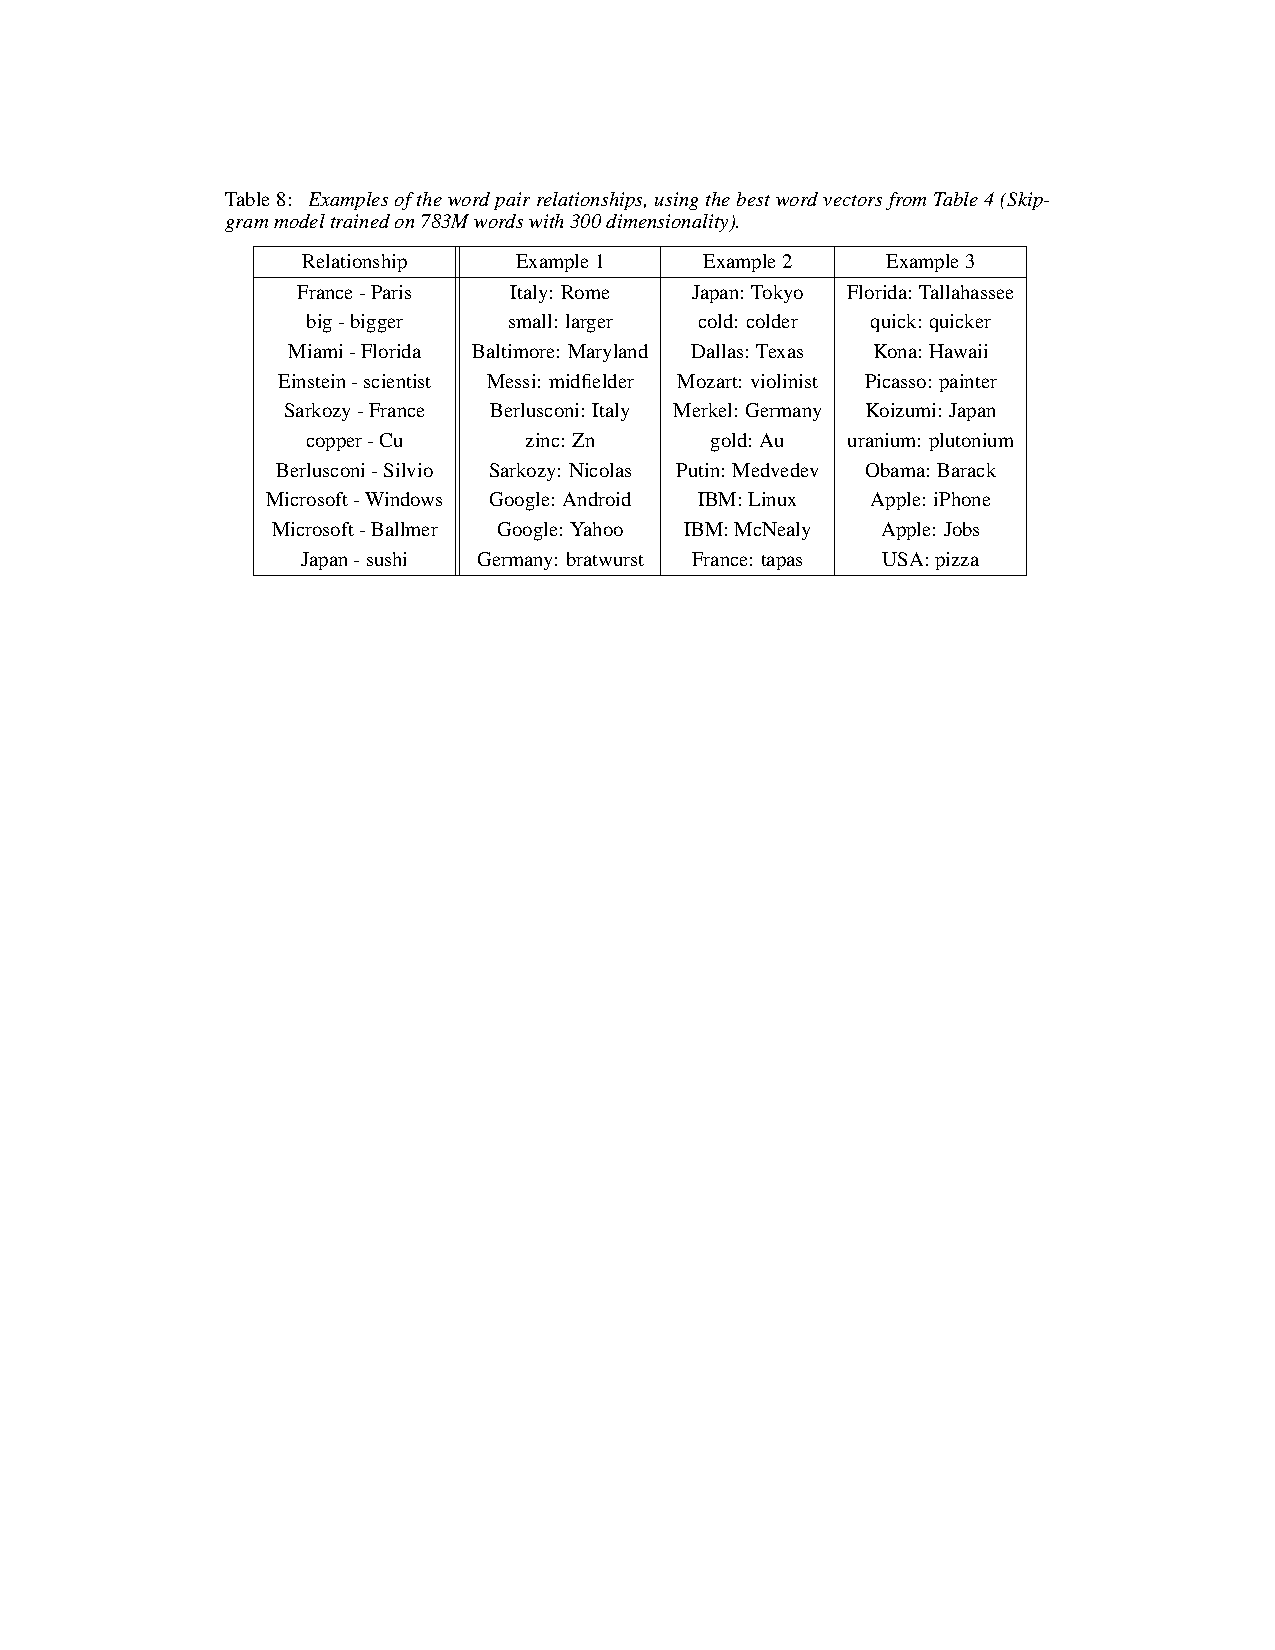
\includegraphics[width=\linewidth]{mikolov-example-relationships}
\end{frame}

\section{Pennington et al 2014: GloVe: Global Vectors for Word Representation}

\begin{frame}

\begin{itemize}
\item a szóanalógiás feladat: King - Queen = Man - Woman

\item vektorok esetén szépen elegánsan vektoriális kivonás

\item erre a feladatra fókuszálva dolgozzák ki a glove modellt
\end{itemize}
\end{frame}

\begin{frame}
\begin{description}
\item[megfigyelés 1:]
\(i, j, k\) szavak, \(P()\) valószínűségek: \(\frac{P(k|i)}{P(k|j)} >> 1\), ha \(k\) jelentése kapcsolatos az \(i, j\) szavakkal, de az \(i\) szóra jellemző, \(j\)-re nem; és közel van 1-hez, ha inadekvát. Tehát a \(w_i-w_j\) szóvektorok különbsége a valószínűségük hányadosaival lehet arányos a modellben.

\item[megfigyelés 2:]
\(w_i-w_j\) különbség és a \(w_k\) próbaszó (probe word) vektorokra szimmetrikus is lehetne a modell (mert a szó-kontextusszó viszony szimmetrikus)

\item[megfigyelés 3:]
a valószínűségek skalárok, a szóvektorok vektorok, de a két vektor skaláris szorzatát kipróbálhatnánk
\end{description}
\end{frame}

\begin{frame}
levezethető, hogy ilyen tulajdonságokkal rendelkezik ez az egyszerű modell:
\[ w_i \times w_k + b = \log(X_{ik}) \]

a modell betanításához (a \(w_i\) vektorok kiszámításához) a legkisebb négyzetek megfelelő
(a glove-ban még egy súlyfüggvénnyel szorzunk, ami kiegyenlíti a szógyakoriságbeli nagyságrendi különbségeket)

a modell szerencsére a \(|V|^2\)-nél sokkal jobban méretezhető, mert az együttes előfordulások eloszlása nem egyenletes, hanem hatványtörvény szerinti (~ ritka mátrix; polinomiálisan kevesebb számítás szükséges)
\end{frame}

\begin{frame}
\frametitle{Eredmények} 
\textcolor{red}{világverő :)}
\end{frame}
\end{document}

